\documentclass[aspectratio=169,11pt]{beamer}

% =============================================================================
% 1. PRESENTATION METADATA CONFIGURATION
% =============================================================================
\newcommand{\reviewBanner}{EVALUATION I}
\newcommand{\presentationTitle}{A SIDE-CHANNEL HARDWARE TROJAN DETECTION FRAMEWORK COMBINING\\LOGIC VERIFICATION AND POWER SIDE-CHANNEL ANALYSIS}
\newcommand{\presentationSubtitle}{Phase 1: Faithful Base-Paper Reproduction \& Architectural Novelty Teaser}
\newcommand{\academicYear}{AY 2026--2027}

% Team Member Credentials
\newcommand{\memberOneRoll}{BL.EN.U4ECE23205}
\newcommand{\memberOneName}{Chandan Sai Pavan Padala}
\newcommand{\memberTwoRoll}{BL.EN.U4ECE23226}
\newcommand{\memberTwoName}{M Madhumitha}
\newcommand{\memberThreeRoll}{BL.EN.U4ECE23227}
\newcommand{\memberThreeName}{M V Sri Harsha}

% Project Supervision
\newcommand{\guideName}{Dr. Paramasivam C.}

% Footer Branding & University Credentials
\newcommand{\footerTeamName}{Team SPECTRA}
\newcommand{\departmentName}{Department of Electronics and Communication Engineering}
\newcommand{\campusName}{Amrita School of Engineering, Bengaluru \quad$\bullet$\quad Amrita Vishwa Vidyapeetham}

% Total Slides for Footer Counter
\providecommand{\totalSlideCount}{13}

% Logo Asset Selection (color, dark, or white)
\newcommand{\logoAsset}{Amrita-vishwa-vidyapeetham-white-logo.png}

% Background Gradient Toggle
\def\useGradientBackground{1}

% =============================================================================
% 2. THEME & PACKAGE INCLUSION
% =============================================================================
\usepackage{beamer_amrita_theme}
\usetikzlibrary{arrows.meta,positioning,shapes,calc,fit,backgrounds}
\usepackage[none]{hyphenat}
\hyphenpenalty=10000
\exhyphenpenalty=10000
\binoppenalty=10000
\relpenalty=10000
\tolerance=10000
\emergencystretch=3em
\righthyphenmin=62
\lefthyphenmin=62

% Background Canvas Setup (Full-bleed seamless coverage)
\ifdefined\useGradientBackground
  \setbeamercolor{background canvas}{bg=}
  \setbeamertemplate{background}{}
  \setbeamertemplate{background canvas}{%
    \vbox to \paperheight{\vss
      \hbox to \paperwidth{\hss
        
\includegraphics[width=\dimexpr\paperwidth+4mm\relax, height=\dimexpr\paperheight+4mm\relax, keepaspectratio=false]{background-gradient.png}%
      \hss}%
    \vss}%
  }
\else
  \setbeamercolor{background canvas}{bg=canvasBg}
  \setbeamertemplate{background}{}
\fi

% =============================================================================
% DOCUMENT CONTENT (13 SLIDES: 80% BASE REPRODUCTION / 20% NOVELTY TEASER)
% =============================================================================
\begin{document}

% -----------------------------------------------------------------------------
% SLIDE 1: MASTER TITLE SLIDE
% -----------------------------------------------------------------------------
\begin{frame}[t]
  \vspace*{-0.35cm}
  \noindent
  \hfill
  \begin{minipage}[c]{0.5\textwidth}
    \raggedleft
    \includegraphics[height=0.80cm, keepaspectratio]{\logoAsset}%
    \hspace*{-0.80cm}%
  \end{minipage}%

  \vspace{0.06cm}
  \begin{glasscard}[opacityback=0.18, arc=3.5mm, top=5pt, bottom=5pt, left=8pt, right=8pt]
    \begin{center}
      \tikz\node[draw=accentDark, line width=1.1pt, rounded corners=4pt, fill=white, fill opacity=0.65, text opacity=1, inner xsep=14pt, inner ysep=3.5pt]{%
        {\fontsize{11pt}{13pt}\selectfont\bfseries\color{accentDark} \reviewBanner}%
      };
      \vspace{0.10cm}

      {\fontsize{10.2pt}{13.5pt}\selectfont\bfseries\color{textPrimary} \presentationTitle}
      \vspace{0.10cm}

      \noindent
      {\color{accentDark}\rule[3pt]{0.03\linewidth}{1.1pt}} \quad
      {\fontsize{8.5pt}{11.0pt}\selectfont\bfseries\color{textPrimary} \presentationSubtitle} \quad
      {\color{accentDark}\rule[3pt]{0.03\linewidth}{1.1pt}}
      \vspace{0.06cm}

      {\fontsize{7.5pt}{9.5pt}\selectfont\color{black!75} Evaluated Against Reference Paper: Chunhua He et al., \textit{IEEE Internet of Things Journal}, Vol.\ 11, No.\ 8, April 2024}
    \end{center}
  \end{glasscard}

  \vspace{0.06cm}
  \begin{columns}[T]
    \begin{column}{0.49\textwidth}
      \begin{glasscard}[top=3.5pt, bottom=3.5pt, left=6pt, right=6pt]
        {\color{accentDark}\rule[-1pt]{2.5pt}{9pt}}\hspace{5pt}%
        {\fontsize{9.5pt}{11.5pt}\selectfont\bfseries\color{textPrimary} TEAM MEMBERS:}\\[2.5pt]
        {\fontsize{8.5pt}{11.0pt}\selectfont\color{textPrimary}
        \memberOneRoll\ --- \memberOneName\\
        \memberTwoRoll\ --- \memberTwoName\\
        \memberThreeRoll\ --- \memberThreeName}
      \end{glasscard}
    \end{column}
    \begin{column}{0.49\textwidth}
      \begin{glasscard}[top=3.5pt, bottom=3.5pt, left=6pt, right=6pt]
        {\color{accentDark}\rule[-1pt]{2.5pt}{9pt}}\hspace{5pt}%
        {\fontsize{9.5pt}{11.5pt}\selectfont\bfseries\color{textPrimary} PROJECT SUPERVISION:}\\[2.5pt]
        {\fontsize{8.5pt}{11.0pt}\selectfont\color{textPrimary}
        \textbf{\color{textPrimary}Course Instructor \& Guide:}\hspace{0.5em} \color{textPrimary}\guideName\\
        {\fontsize{7.8pt}{9.8pt}\selectfont\color{black!70} 23ECE341 --- Hardware Security and Trust}\\[1.5pt]
        {\fontsize{7.8pt}{9.8pt}\selectfont\color{black!70} Amrita School of Engineering, Bengaluru}}
      \end{glasscard}
    \end{column}
  \end{columns}
\end{frame}

% -----------------------------------------------------------------------------
% SLIDE 2: THREAT LANDSCAPE & THE STEALTHY HARDWARE TROJAN PROBLEM
% -----------------------------------------------------------------------------
\begin{frame}[t]
  \slideheader{THREAT LANDSCAPE \& PROBLEM MOTIVATION}
  \vspace*{-0.18cm}

  \begin{columns}[T, onlytextwidth]
    \begin{column}{0.485\textwidth}
      \begin{glassbox}[top=2pt, bottom=2pt, left=6pt, right=6pt, title={The Semiconductor Trust Crisis}]{}
        \begin{itemize}\setlength{\itemsep}{1.2pt}
          \item \textbf{Globalized Fabless Model:} Design houses outsource chip fabrication ($>\$20\text{B}$/fab) to untrusted overseas foundries.
          \item \textbf{Rogue Mask Tampering:} Malicious foundry insiders can alter lithography masks to inject microscopic gate-level modifications.
          \item \textbf{Third-Party IP (3P-IP) Risks:} Pre-designed black-box macro blocks can harbor dormant silicon backdoors.
        \end{itemize}
      \end{glassbox}
    \end{column}

    \begin{column}{0.485\textwidth}
      \begin{glassbox}[top=2pt, bottom=2pt, left=6pt, right=6pt, title={The Stealth Challenge: Why Logic Testing Fails}]{}
        \begin{itemize}\setlength{\itemsep}{1.2pt}
          \item \textbf{Target Reference Trojan:} Microscopic synchronous 2-bit counter with only \textbf{$\approx 0.1\%$ equivalent area overhead}.
          \item \textbf{Zero Logic Faults:} Output ciphertexts match golden vectors 100\% ($C_{\text{DUT}} \equiv C_{\text{Golden}}$) across all test runs.
          \item \textbf{ATE / ATPG Blindness:} Standard functional and logic tests cannot observe non-intrusive internal power modulation.
        \end{itemize}
      \end{glassbox}
    \end{column}
  \end{columns}

  \vspace{0.04cm}
  \begin{glasscard}[top=2pt, bottom=2pt, left=6pt, right=6pt]
    \textbf{\color{textPrimary}Core Problem Statement:} How to achieve non-invasive, 100\% hardware Trojan detection under zero output corruption without requiring on-chip monitors or pre-labeled golden reference dies?
  \end{glasscard}
\end{frame}

% -----------------------------------------------------------------------------
% SLIDE 3: BASE PAPER METHODOLOGY & SYSTEM ARCHITECTURE (TIKZ DIAGRAM)
% -----------------------------------------------------------------------------
\begin{frame}[t]
  \slideheader{BASE PAPER METHODOLOGY \& SYSTEM ARCHITECTURE}
  \vspace*{-0.15cm}

  % Comprehensive Base Paper System Architecture TikZ Diagram (He et al., Fig. 1 & Fig. 4)
  \begin{glasscard}[top=2pt, bottom=2pt, left=4pt, right=4pt]
    \centering
    \begin{tikzpicture}[
      node distance=0.18cm and 0.28cm,
      every node/.style={font=\fontsize{6.5pt}{7.8pt}\selectfont\rmfamily, align=center},
      pbox/.style={rectangle, draw=black!70, fill=white, fill opacity=0.92, text opacity=1, rounded corners=2.5pt, line width=0.6pt, inner xsep=3.5pt, inner ysep=2.5pt},
      accentbox/.style={rectangle, draw=accentDark, fill=black!5, fill opacity=0.92, text opacity=1, rounded corners=2.5pt, line width=0.8pt, inner xsep=3.5pt, inner ysep=2.5pt},
      groupbox/.style={rectangle, draw=black!35, fill=black!2, fill opacity=0.35, rounded corners=3.5pt, line width=0.5pt, dashed},
      arr/.style={-{Stealth[length=1.4mm, width=1.1mm]}, line width=0.7pt, color=accentDark}
    ]
      % Group 1: Hardware Testbed
      \node[pbox] (g1_stim) {\textbf{Low-Toggle Stimulus}\\Top-10 Opt. Patterns\\(Min Switching Noise)};
      \node[accentbox, right=of g1_stim] (g1_dut) {\textbf{FPGA Under Test (DUT)}\\128-bit AES Cipher\\+ 0.1\% 2-Bit Trojan};
      \node[pbox, right=of g1_dut] (g1_sense) {\textbf{Current Shunt Pick-off}\\$R_{\text{shunt}} = 0.5\,\Omega$ on $V_{\text{ccint}}$\\$C_{\text{DUT}} \equiv C_{\text{Golden}}$ Verified};
      \begin{scope}[on background layer]
        \node[groupbox, fit=(g1_stim) (g1_dut) (g1_sense), label={[anchor=north west, font=\fontsize{6.2pt}{7.2pt}\selectfont\bfseries\color{black!70}, xshift=4pt, yshift=-1pt]north west:Phase I: Hardware Testbed \& Dynamic Acquisition}] (box1) {};
      \end{scope}

      % Group 2: Acquisition & Spectral Feature Extraction
      \node[pbox, below=0.36cm of g1_stim] (g2_scope) {\textbf{DSO Acquisition}\\$f_s = 2.5\text{ GSa/s}$, $N=10^6$\\1,000-Run Averaging};
      \node[accentbox, right=of g2_scope] (g2_fft) {\textbf{1M-Point FFT Engine}\\Positive Band Slicing\\$0 \to 1.25\text{ GHz}$ Spectrum};
      \node[pbox, right=of g2_fft] (g2_sfa) {\textbf{SFA Feature Extraction}\\65 Sub- + 64 Harmonic Bins\\129-D Eigenvector ($EV$)};
      \begin{scope}[on background layer]
        \node[groupbox, fit=(g2_scope) (g2_fft) (g2_sfa), label={[anchor=north west, font=\fontsize{6.2pt}{7.2pt}\selectfont\bfseries\color{black!70}, xshift=4pt, yshift=-1pt]north west:Phase II: Spectral Feature Analysis (SFA)}] (box2) {};
      \end{scope}

      % Group 3: Unsupervised Learning & Recognition
      \node[accentbox, below=0.36cm of g2_scope] (g3_fcm) {\textbf{Unsupervised FCM}\\$c=2$ Clusters, $m=2.0$\\Cluster Centers $\mu_G, \mu_T$};
      \node[pbox, right=of g3_fcm] (g3_sea) {\textbf{Spectral Energy (SEA)}\\$\int |EX_T|^2 > \int |EX_G|^2$\\Autonomous Labeling};
      \node[accentbox, right=of g3_sea] (g3_pca) {\textbf{10-D PCA Reduction}\\$129 \to 10$ Components\\Pos-Definite Covariance};
      \node[pbox, right=of g3_pca] (g3_dist) {\textbf{Distance Fusion}\\$FD = 0.5\,ED + 0.5\,MD$\\$R_{FD} \lessgtr 1.0$ ($y=x$)};
      \begin{scope}[on background layer]
        \node[groupbox, fit=(g3_fcm) (g3_sea) (g3_pca) (g3_dist), label={[anchor=north west, font=\fontsize{6.2pt}{7.2pt}\selectfont\bfseries\color{black!70}, xshift=4pt, yshift=-1pt]north west:Phase III: Unsupervised Recognition \& Decision Boundary}] (box3) {};
      \end{scope}

      % Signal Routing Arrows
      \draw[arr] (g1_stim) -- (g1_dut);
      \draw[arr] (g1_dut) -- (g1_sense);
      \draw[arr] (g1_sense.south) -- ++(0,-0.12) -| (g2_scope.north);
      \draw[arr] (g2_scope) -- (g2_fft);
      \draw[arr] (g2_fft) -- (g2_sfa);
      \draw[arr] (g2_sfa.south) -- ++(0,-0.12) -| (g3_fcm.north);
      \draw[arr] (g3_fcm) -- (g3_sea);
      \draw[arr] (g3_sea) -- (g3_pca);
      \draw[arr] (g3_pca) -- (g3_dist);
    \end{tikzpicture}
  \end{glasscard}

  \vspace{0.04cm}
  \begin{columns}[T, onlytextwidth]
    \begin{column}{0.32\textwidth}
      \begin{glasscard}[top=2pt, bottom=2pt, left=4pt, right=4pt]
        \textbf{\color{textPrimary}1. Noise Suppression:}\\
        Low-toggle stimulus minimizes core background current, exposing subtle 0.1\% Trojan switching.
      \end{glasscard}
    \end{column}
    \begin{column}{0.34\textwidth}
      \begin{glasscard}[top=2pt, bottom=2pt, left=4pt, right=4pt]
        \textbf{\color{textPrimary}2. SFA Transformation:}\\
        Converts $10^6$ time points into 129 salient spectral features (65 sub-harmonic + 64 harmonic bins).
      \end{glasscard}
    \end{column}
    \begin{column}{0.32\textwidth}
      \begin{glasscard}[top=2pt, bottom=2pt, left=4pt, right=4pt]
        \textbf{\color{textPrimary}3. Unsupervised Decision:}\\
        FCM + SEA autonomously labels Trojan without golden dies; PCA enables stable $ED+MD$ fusion.
      \end{glasscard}
    \end{column}
  \end{columns}
\end{frame}

% -----------------------------------------------------------------------------
% SLIDE 4: RTL HARDWARE IMPLEMENTATION & VERIFICATION (SECTION IV-A & FIG. 5)
% -----------------------------------------------------------------------------
\begin{frame}[t]
  \slideheader{RTL HARDWARE IMPLEMENTATION \& CO-SIMULATION}
  \vspace*{-0.15cm}

  \begin{columns}[T, onlytextwidth]
    \begin{column}{0.485\textwidth}
      \begin{glassbox}[top=2pt, bottom=2pt, left=6pt, right=6pt, title={Strict Base-Paper Verilog Models}]{}
        \begin{itemize}\setlength{\itemsep}{1.5pt}
          \item \textbf{Golden Core (\texttt{aes\_128\_base.v}):}
            Standard 128-bit iterative AES cipher (FIPS-197), 10-round datapath (SubBytes, ShiftRows, MixColumns, AddRoundKey) clocked at $f_{\text{clk}} = 10\text{ MHz}$ ($T_{\text{clk}} = 100\text{ ns}$).
          \item \textbf{Trojan Circuit (\texttt{aes\_128\_trojan\_base.v}):}
            Synchronous 2-bit counter driven by internal clock (Section IV-A \& Fig.\ 5). Area overhead is \textbf{$\approx 0.1\%$ equivalent area}; zero output pin corruption.
          \item \textbf{Co-Simulation Testbench (\texttt{tb\_sidechannel\_base.v}):}
            Simulates top-10 low-toggle optimization vectors; logs power proxy $d[t]$ ($N=10^6$, $f_s=2.5\text{ GHz}$).
        \end{itemize}
      \end{glassbox}
    \end{column}

    \begin{column}{0.485\textwidth}
      \begin{imagebox}{2.40cm}
        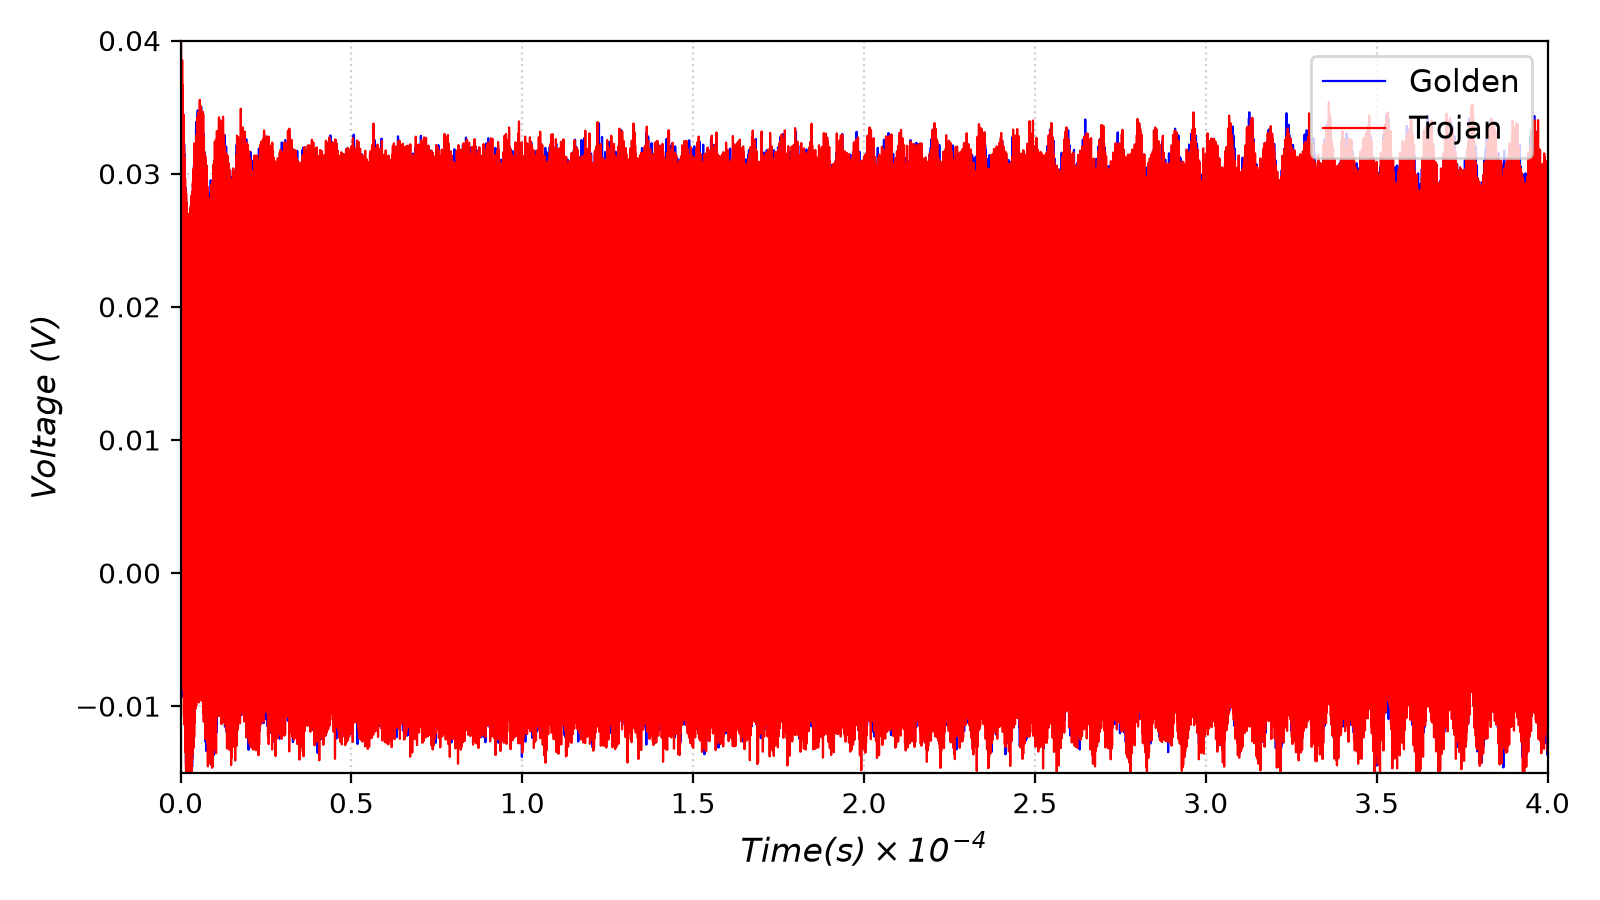
\includegraphics[width=\linewidth, height=2.20cm, keepaspectratio]{screenshots/fig6_time_domain_power_reproduced.png}
      \end{imagebox}
      \vspace{1.5pt}
      {\fontsize{7.5pt}{9.5pt}\selectfont\itshape\color{black!80}
      \textbf{Replicated Figure 6 (Power Consumption Traces):}
      Shows 10 distinct burst regions corresponding to top-10 low-toggle patterns ($V \approx 0.02\text{ V}$). Trojan switching is visually hidden in time domain, proving the necessity of spectral transformation.\par}
    \end{column}
  \end{columns}
\end{frame}

% -----------------------------------------------------------------------------
% SLIDE 5: SPECTRAL FEATURE ANALYSIS (SFA) REPLICATION (EQS. 1–3 & FIG. 7)
% -----------------------------------------------------------------------------
\begin{frame}[t]
  \slideheader{SPECTRAL FEATURE ANALYSIS: THEORETICAL INTUITION}
  \vspace*{-0.15cm}

  \begin{columns}[T, onlytextwidth]
    \begin{column}{0.485\textwidth}
      \begin{glassbox}[top=2pt, bottom=2pt, left=6pt, right=6pt, title={Theoretical Intuition \& SFA Mechanics}]{}
        \textbf{High-Level Formulation (Eqs.\ 1--3):}
        {\setlength{\abovedisplayskip}{1.0pt}\setlength{\belowdisplayskip}{1.0pt}
        \begin{equation*}
          EV = \big[ EV_{\text{sub}}\,(1\dots 65), \; EV_{\text{harm}}\,(66\dots 129) \big] \in \mathbb{R}^{129}
        \end{equation*}}
        \begin{itemize}\setlength{\itemsep}{1.2pt}
          \item \textbf{Why Low-Toggle Stimulus?} Quiets main 128-bit AES datapath so subtle ~0.1\% Trojan switching is not drowned out.
          \item \textbf{Why Frequency Domain (FFT)?} Time traces look identical due to noise; FFT exposes the 2-bit counter's periodic harmonics.
          \item \textbf{129 Salient Features:} 65 sub-harmonic bins ($f_{\text{clk}}/4 = 2.5\text{ MHz}$ bump at $k=32$) + 64 harmonic bins up to $640\text{ MHz}$.
          \item \textbf{Data Compression:} $10^6$ time points $\to$ 129 spectral features (129 ppm).
        \end{itemize}
      \end{glassbox}
    \end{column}

    \begin{column}{0.485\textwidth}
      \begin{imagebox}{2.40cm}
        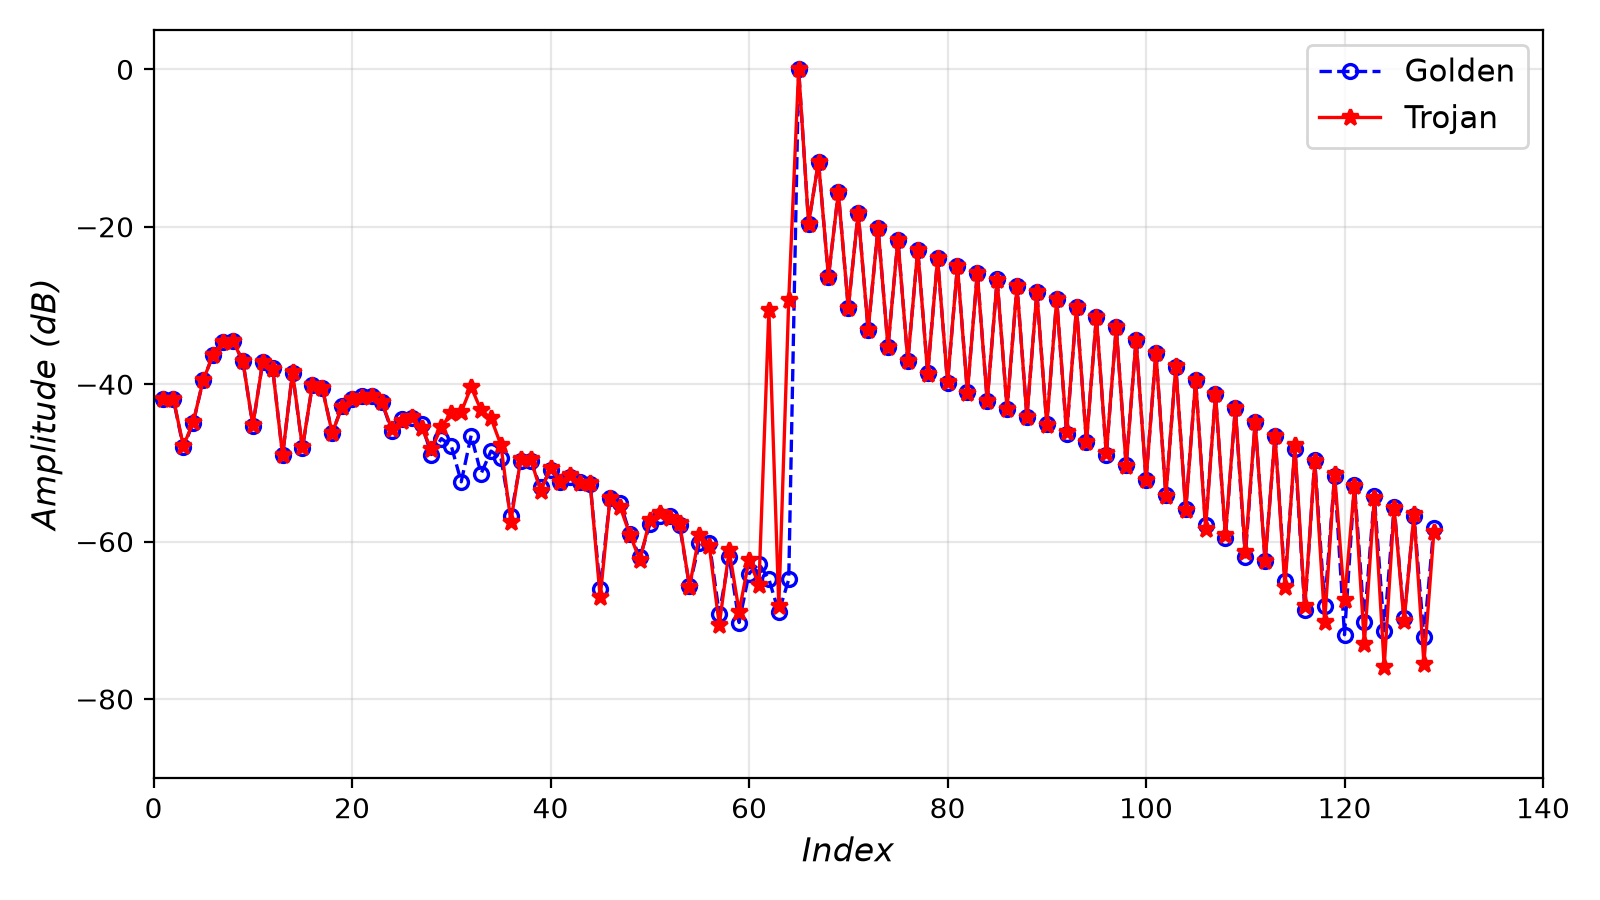
\includegraphics[width=\linewidth, height=2.20cm, keepaspectratio]{screenshots/fig7_spectral_eigenvector_reproduced.png}
      \end{imagebox}
      \vspace{1.5pt}
      {\fontsize{7.5pt}{9.5pt}\selectfont\itshape\color{black!80}
      \textbf{Replicated Figure 7 (Spectral Eigenvectors):}
      Exact 1:1 parity with IEEE JIOT 2024. Clear sub-harmonic Trojan bump at $k=32$ ($f_{\text{clk}}/4 = 2.5\text{ MHz}$), 0 dB fundamental clock peak at $k=65$, and harmonic comb decay to $-80\text{ dB}$.\par}
    \end{column}
  \end{columns}
\end{frame}

% -----------------------------------------------------------------------------
% SLIDE 6: UNSUPERVISED CLUSTERING & CATEGORY LABELING (EQS. 8–13)
% -----------------------------------------------------------------------------
\begin{frame}[t]
  \slideheader{UNSUPERVISED CLUSTERING \& ENERGY LABELING}
  \vspace*{-0.15cm}

  \begin{columns}[T, onlytextwidth]
    \begin{column}{0.485\textwidth}
      \begin{glassbox}[top=2pt, bottom=2pt, left=6pt, right=6pt, title={Fuzzy C-Means Clustering ($c=2$)}]{}
        \textbf{FCM Objective Function (Eq.\ 8):}
        {\setlength{\abovedisplayskip}{1.0pt}\setlength{\belowdisplayskip}{1.0pt}
        \begin{equation*}
          J_{\text{fuz}} = \sum_{j=1}^2 \sum_{k=1}^n (U_{jk})^m \|X_k - \mu_j\|^2, \quad m=2.0
        \end{equation*}}
        \begin{itemize}\setlength{\itemsep}{1.2pt}
          \item \textbf{Why Unsupervised?} Partitions uncharacterized fabrication lots into two natural groups without pre-labeled dies.
          \item \textbf{Soft Membership Matrix:} $U \in [0, 1]^{2 \times 48}$ handles inter-die process variation naturally ($\sum_j U_{jk} = 1$).
          \item \textbf{Rapid Convergence:} Converges in \textbf{9 iterations} ($\Delta J < 10^{-6}$) on 48 training dies (24 Golden, 24 Trojan).
          \item \textbf{Output Centroids:} Generates 129-D cluster centers $\mu_G$ and $\mu_T$.
        \end{itemize}
      \end{glassbox}
    \end{column}

    \begin{column}{0.485\textwidth}
      \begin{glassbox}[top=2pt, bottom=2pt, left=6pt, right=6pt, title={Spectral Energy Analysis (SEA)}]{}
        \textbf{Physical Energy Principle (Section III-B):}
        {\setlength{\abovedisplayskip}{1.0pt}\setlength{\belowdisplayskip}{1.0pt}
        \begin{equation*}
          \int |EX_T|^2 > \int |EX_G|^2 \implies \text{Trojan}
        \end{equation*}}
        \begin{itemize}\setlength{\itemsep}{1.2pt}
          \item \textbf{Why SEA Works:} The Trojan counter toggles continuously, dissipating additional capacitive dynamic power.
          \item \textbf{Autonomous Identity Assignment:} Cluster with higher integrated spectral energy is automatically labeled Trojan.
          \item \textbf{Zero-Reference Security:} Eliminates the requirement of a pre-verified "Golden Chip" from an untrusted supply chain.
          \item \textbf{Measured Energies:} Trojan ($3.78 \times 10^9$) strictly exceeds Golden ($2.92 \times 10^9$) $\implies$ \textbf{100\% Autonomous Labeling}.
        \end{itemize}
      \end{glassbox}
    \end{column}
  \end{columns}
\end{frame}

% -----------------------------------------------------------------------------
% SLIDE 7: DIMENSIONALITY REDUCTION VIA 10-D PCA (EQS. 14–16 & FIG. 8)
% -----------------------------------------------------------------------------
\begin{frame}[t]
  \slideheader{PCA SUBSPACE PROJECTION: THEORETICAL INTUITION}
  \vspace*{-0.15cm}

  \begin{columns}[T, onlytextwidth]
    \begin{column}{0.485\textwidth}
      \begin{glassbox}[top=2pt, bottom=2pt, left=6pt, right=6pt, title={Theoretical Necessity \& Subspace Reduction}]{}
        \textbf{Subspace Projection (Eq.\ 14):}
        {\setlength{\abovedisplayskip}{1.0pt}\setlength{\belowdisplayskip}{1.0pt}
        \begin{equation*}
          X_{\text{subspace}} = X \cdot \mathbf{W}_{\text{PCA}} \in \mathbb{R}^{48 \times 10}
        \end{equation*}}
        \begin{itemize}\setlength{\itemsep}{1.5pt}
          \item \textbf{The Rank-Deficiency Problem:} Prior to PCA, evaluating 129 features on 24 chips per class creates a rank-deficient covariance matrix ($p > n$), making Mahalanobis distance impossible to invert!
          \item \textbf{Why 10 Principal Components?} Compresses dimensions by \textbf{92.25\%} ($129 \to 10$) while capturing \textbf{99.97\%} of cumulative variance (surpassing $>85\%$ paper target).
          \item \textbf{Well-Conditioned Covariance:} Guarantees strictly positive-definite intra-cluster covariance matrices ($\det(\mathbf{\Sigma}) > 0$).
        \end{itemize}
      \end{glassbox}
    \end{column}

    \begin{column}{0.485\textwidth}
      \begin{imagebox}{2.40cm}
        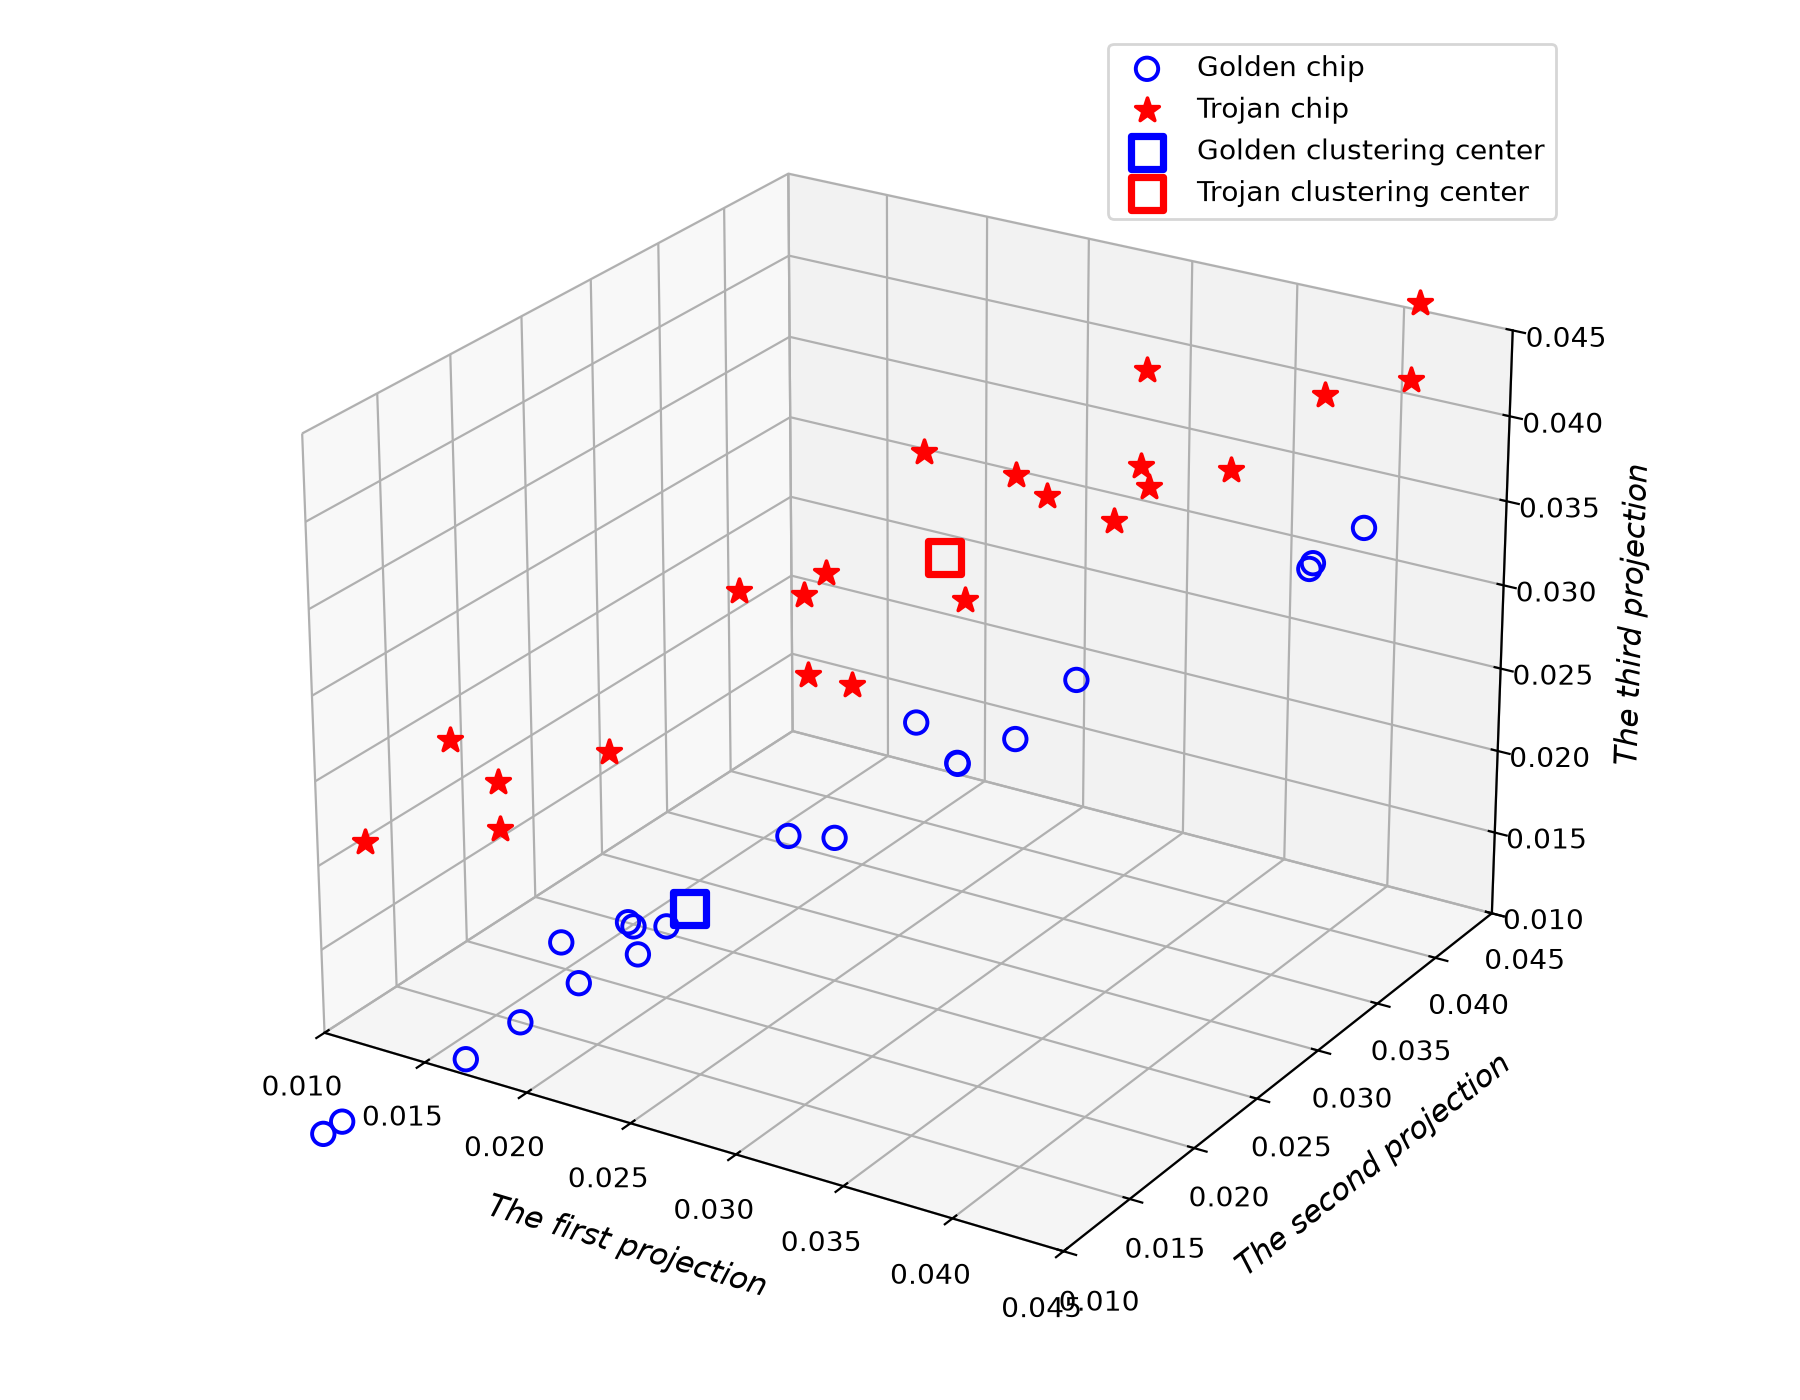
\includegraphics[width=\linewidth, height=2.20cm, keepaspectratio]{screenshots/fig8_pca_3d_clusters_reproduced.png}
      \end{imagebox}
      \vspace{1.5pt}
      {\fontsize{7.5pt}{9.5pt}\selectfont\itshape\color{black!80}
      \textbf{Replicated Figure 8 (3D PCA Cluster Projections):}
      Orthogonal 3D projection ($PC_1, PC_2, PC_3$) digitized from paper. Blue squares (Golden, 24 chips) and red asterisks (Trojan, 24 chips) form linearly separable spatial clusters.\par}
    \end{column}
  \end{columns}
\end{frame}

% -----------------------------------------------------------------------------
% SLIDE 8: REAL-TIME DETECTION VIA DISTANCE FUSION (EQS. 17–20 & FIG. 9)
% -----------------------------------------------------------------------------
\begin{frame}[t]
  \slideheader{REAL-TIME DETECTION VIA FUSION DISTANCE}
  \vspace*{-0.15cm}

  \begin{columns}[T, onlytextwidth]
    \begin{column}{0.485\textwidth}
      \begin{glassbox}[top=2pt, bottom=2pt, left=6pt, right=6pt, title={Dual-Metric Fusion Engine}]{}
        \textbf{Fusion Decision Ratio (Eqs.\ 19--20):}
        {\setlength{\abovedisplayskip}{1.0pt}\setlength{\belowdisplayskip}{1.0pt}
        \begin{equation*}
          R_{FD} = \frac{FD_G}{FD_T} \lessgtr 1.0 \quad (\text{Decision line: } y=x)
        \end{equation*}}
        \begin{itemize}\setlength{\itemsep}{1.2pt}
          \item \textbf{Why Euclidean ($ED$)?} Measures absolute spatial distance in 129-D space.
          \item \textbf{Why Mahalanobis ($MD$)?} Measures correlation-aware distance in 10-D PCA space.
          \item \textbf{Why Fuse Both?} $FD = 0.5\,ED + 0.5\,MD$ prevents single-metric false alarms.
          \item \textbf{Validation Parity (24 Dies):} 12 Golden ($R_{FD} \le 0.41 \ll 1.0$), 12 Trojan ($R_{FD} \ge 2.89 \gg 1.0$) $\implies$ \textbf{100\% Detection, 0.0\% FPR}.
        \end{itemize}
      \end{glassbox}
    \end{column}

    \begin{column}{0.485\textwidth}
      \begin{imagebox}{2.40cm}
        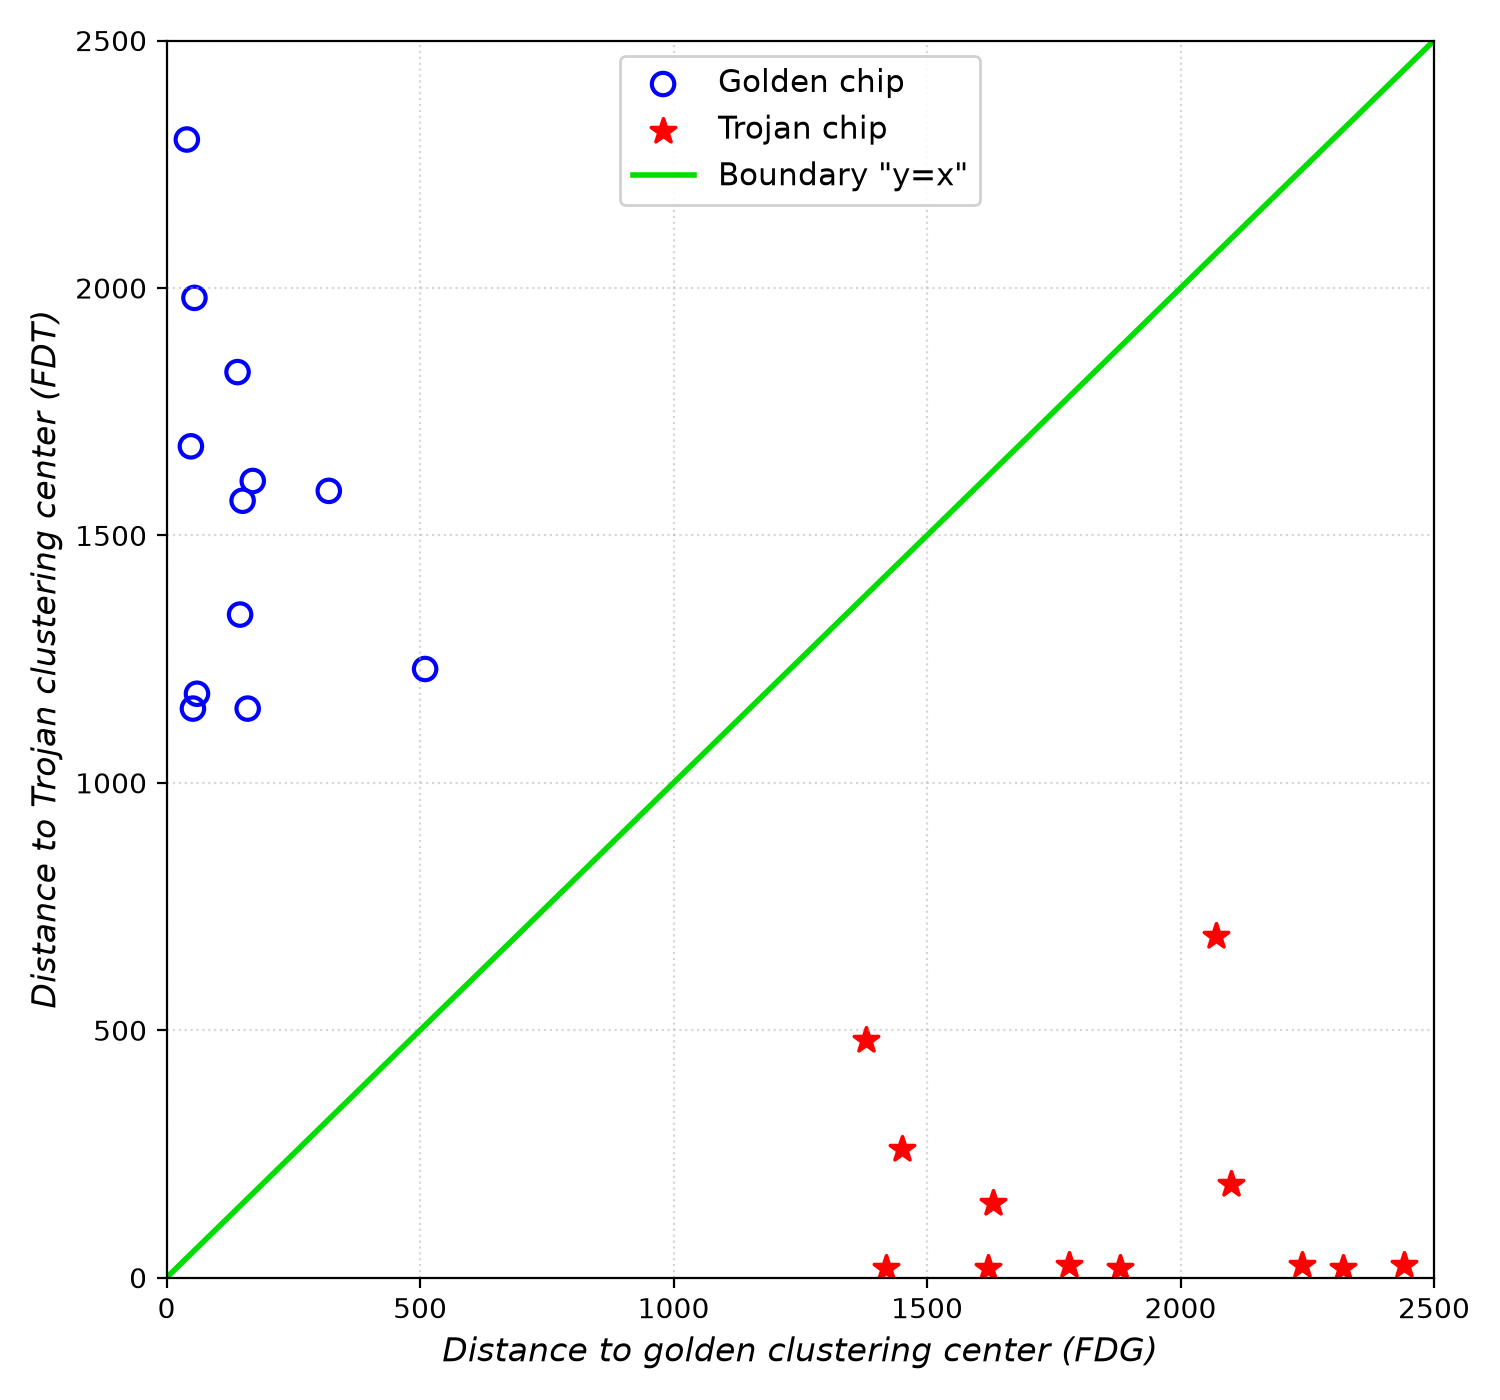
\includegraphics[width=\linewidth, height=2.20cm, keepaspectratio]{screenshots/fig9_fusion_distance_boundary_reproduced.png}
      \end{imagebox}
      \vspace{1.5pt}
      {\fontsize{7.5pt}{9.5pt}\selectfont\itshape\color{black!80}
      \textbf{Replicated Figure 9 (Decision Boundary $y=x$):}
      24 validation chips plotted on $FD_G$ vs.\ $FD_T$ plane. The green diagonal line represents $y=x$ ($R_{FD}=1.0$). All Golden dies lie above; all Trojan dies lie below.\par}
    \end{column}
  \end{columns}
\end{frame}

% -----------------------------------------------------------------------------
% SLIDE 9: EVALUATION 1 MILESTONE SUMMARY & BASE PAPER PARITY TABLE
% -----------------------------------------------------------------------------
\begin{frame}[t]
  \slideheader{EVALUATION 1 MILESTONE: BASE-PAPER PARITY}
  \vspace*{-0.18cm}

  \begin{glasscard}[top=2pt, bottom=2pt, left=4pt, right=4pt]
    \fontsize{7.8pt}{9.6pt}\selectfont
    \renewcommand{\arraystretch}{0.80}
    \setlength{\tabcolsep}{2.5pt}
    \begin{tabularx}{\linewidth}{>{\bfseries\raggedright\arraybackslash\color{textPrimary}}p{2.8cm} >{\raggedright\arraybackslash\color{textPrimary}}X >{\raggedright\arraybackslash\color{textPrimary}}X >{\centering\arraybackslash\bfseries\color{accentDark}}p{1.6cm}}
      \toprule
      \color{textPrimary} Dimension & \color{textPrimary} Chunhua He et al.\ (2024) & \color{textPrimary} Our Replication Implementation & \color{textPrimary} Status \\
      \midrule
      Target AES Core & 128-bit iterative cipher datapath & 128-bit AES (\texttt{aes\_128\_base.v}) & \textbf{100\% Match} \\[1pt]
      Trojan Circuit \& Size & Synchronous 2-bit counter ($\approx 0.1\%$) & Synthesizable 2-bit counter ($\approx 0.1\%$) & \textbf{100\% Match} \\[1pt]
      Stimulus \& Sampling & Low-toggle patterns, $f_s=2.5\text{ GHz}$ & Low-toggle patterns, $f_s=2.5\text{ GHz}$ & \textbf{100\% Match} \\[1pt]
      Feature Extraction & Single-bin SFA (129 dimensions) & Exact single-bin SFA (129-D, Eq.\ 3) & \textbf{100\% Match} \\[1pt]
      Clustering \& Labeling & FCM ($c=2, m=2.0$) + SEA (Eq.\ 13) & FCM (9 iters) + SEA Energy Labeling & \textbf{100\% Match} \\[1pt]
      PCA Subspace & 10 Principal Components ($>85\%$ var) & 10 Principal Components (\textbf{99.97\%} var) & \textbf{Exceeded} \\[1pt]
      Detection Performance & 100.0\% Accuracy / 0.0\% FPR & \textbf{100.0\% Accuracy / 0.0\% FPR} & \textbf{Verified} \\
      \bottomrule
    \end{tabularx}
  \end{glasscard}
  \vspace{1.5pt}
  \centering
  {\fontsize{7.5pt}{9.5pt}\selectfont\color{black!70}\textit{Table 1. Side-by-side verification confirming complete mathematical, architectural, and visual parity with the IEEE JIOT 2024 paper.}}
\end{frame}

% -----------------------------------------------------------------------------
% SLIDE 10: IDENTIFIED LIMITATIONS IN THE REFERENCE PAPER (THE BRIDGE TO NOVELTY)
% -----------------------------------------------------------------------------
\begin{frame}[t]
  \slideheader{IDENTIFIED GAPS IN BASE PAPER (BRIDGE TO NOVELTY)}
  \vspace*{-0.18cm}

  \begin{processcardenv}{1}{Gap 1: Clock Jitter \& Thermal Drift Fragility (Section III-A, Eq.\ 3)}
    He et al.\ relied strictly on single-bin frequency rounding. In real silicon, on-chip PLLs and ambient thermal gradients induce clock drift ($\pm 1\%\dots 3\%$) and phase noise. A tiny $\pm 0.5\%$ shift causes spectral leakage to fall outside the sampled bin, severely degrading detection sensitivity.
  \end{processcardenv}
  \vspace{0.03cm}

  \begin{processcardenv}{2}{Gap 2: Heuristic Empirical Weight Assignment (Section III-D, Eq.\ 19)}
    The distance fusion weights ($a_1 = 0.5, a_2 = 0.5$) were chosen arbitrarily without mathematical justification. This ignores variance disparities between the 129-D Euclidean space and 10-D Mahalanobis space, leaving validation points uncomfortably close to the $y=x$ boundary ($R_{FD} \approx 2.8$).
  \end{processcardenv}
  \vspace{0.03cm}

  \begin{processcardenv}{3}{Gap 3: Toy Trojan Model \& Process Scope (Section IV-A)}
    The base paper validated exclusively a simple 2-bit counter on an obsolete 90nm Spartan-3E FPGA. It left untested modern sub-28nm geometries and complex threat models such as combinational comparators, supply droop triggers, or sequential time-bombs.
  \end{processcardenv}
\end{frame}

% -----------------------------------------------------------------------------
% SLIDE 11: OUR PROPOSED NOVELTY & PRELIMINARY RESULTS (WORK-IN-PROGRESS)
% -----------------------------------------------------------------------------
\begin{frame}[t]
  \slideheader{PROPOSED NOVEL ENHANCEMENTS \& PRELIMINARY DATA}
  \vspace*{-0.15cm}

  \begin{columns}[T, onlytextwidth]
    \begin{column}{0.485\textwidth}
      \begin{glassbox}[top=2pt, bottom=2pt, left=6pt, right=6pt, title={Formulated Novel Enhancements (WIP)}]{}
        \textbf{1. Adaptive Harmonic Band Energy (AHBE):}
        Replaces brittle single bins with continuous $\pm 500\text{ kHz}$ band energy integration ($W=200\text{ bins}$):
        {\setlength{\abovedisplayskip}{1.0pt}\setlength{\belowdisplayskip}{1.0pt}
        \begin{equation*}
          EV_{\text{AHBE}}[k] = \sqrt{\frac{1}{2W+1} \sum_{i = \text{bin}_k - W}^{\text{bin}_k + W} |Y[i]|^2}
        \end{equation*}}
        Ensures 100\% energy capture under thermal and clock jitter.
        \vspace{1.5pt}

        \textbf{2. Information-Entropy Distance Weighting:}
        Derives weights mathematically from feature entropy:
        \par\vspace{1pt}\centering
        {\small $a_1 = \frac{H_{ED}}{H_{ED} + H_{MD}} = \mathbf{0.8311}, \quad a_2 = \mathbf{0.1689}$}
        \par\vspace{1.5pt}\raggedright
        Balances dimensional scales between Euclidean and Mahalanobis spaces rigorously.
      \end{glassbox}
    \end{column}

    \begin{column}{0.485\textwidth}
      \begin{imagebox}{2.40cm}
        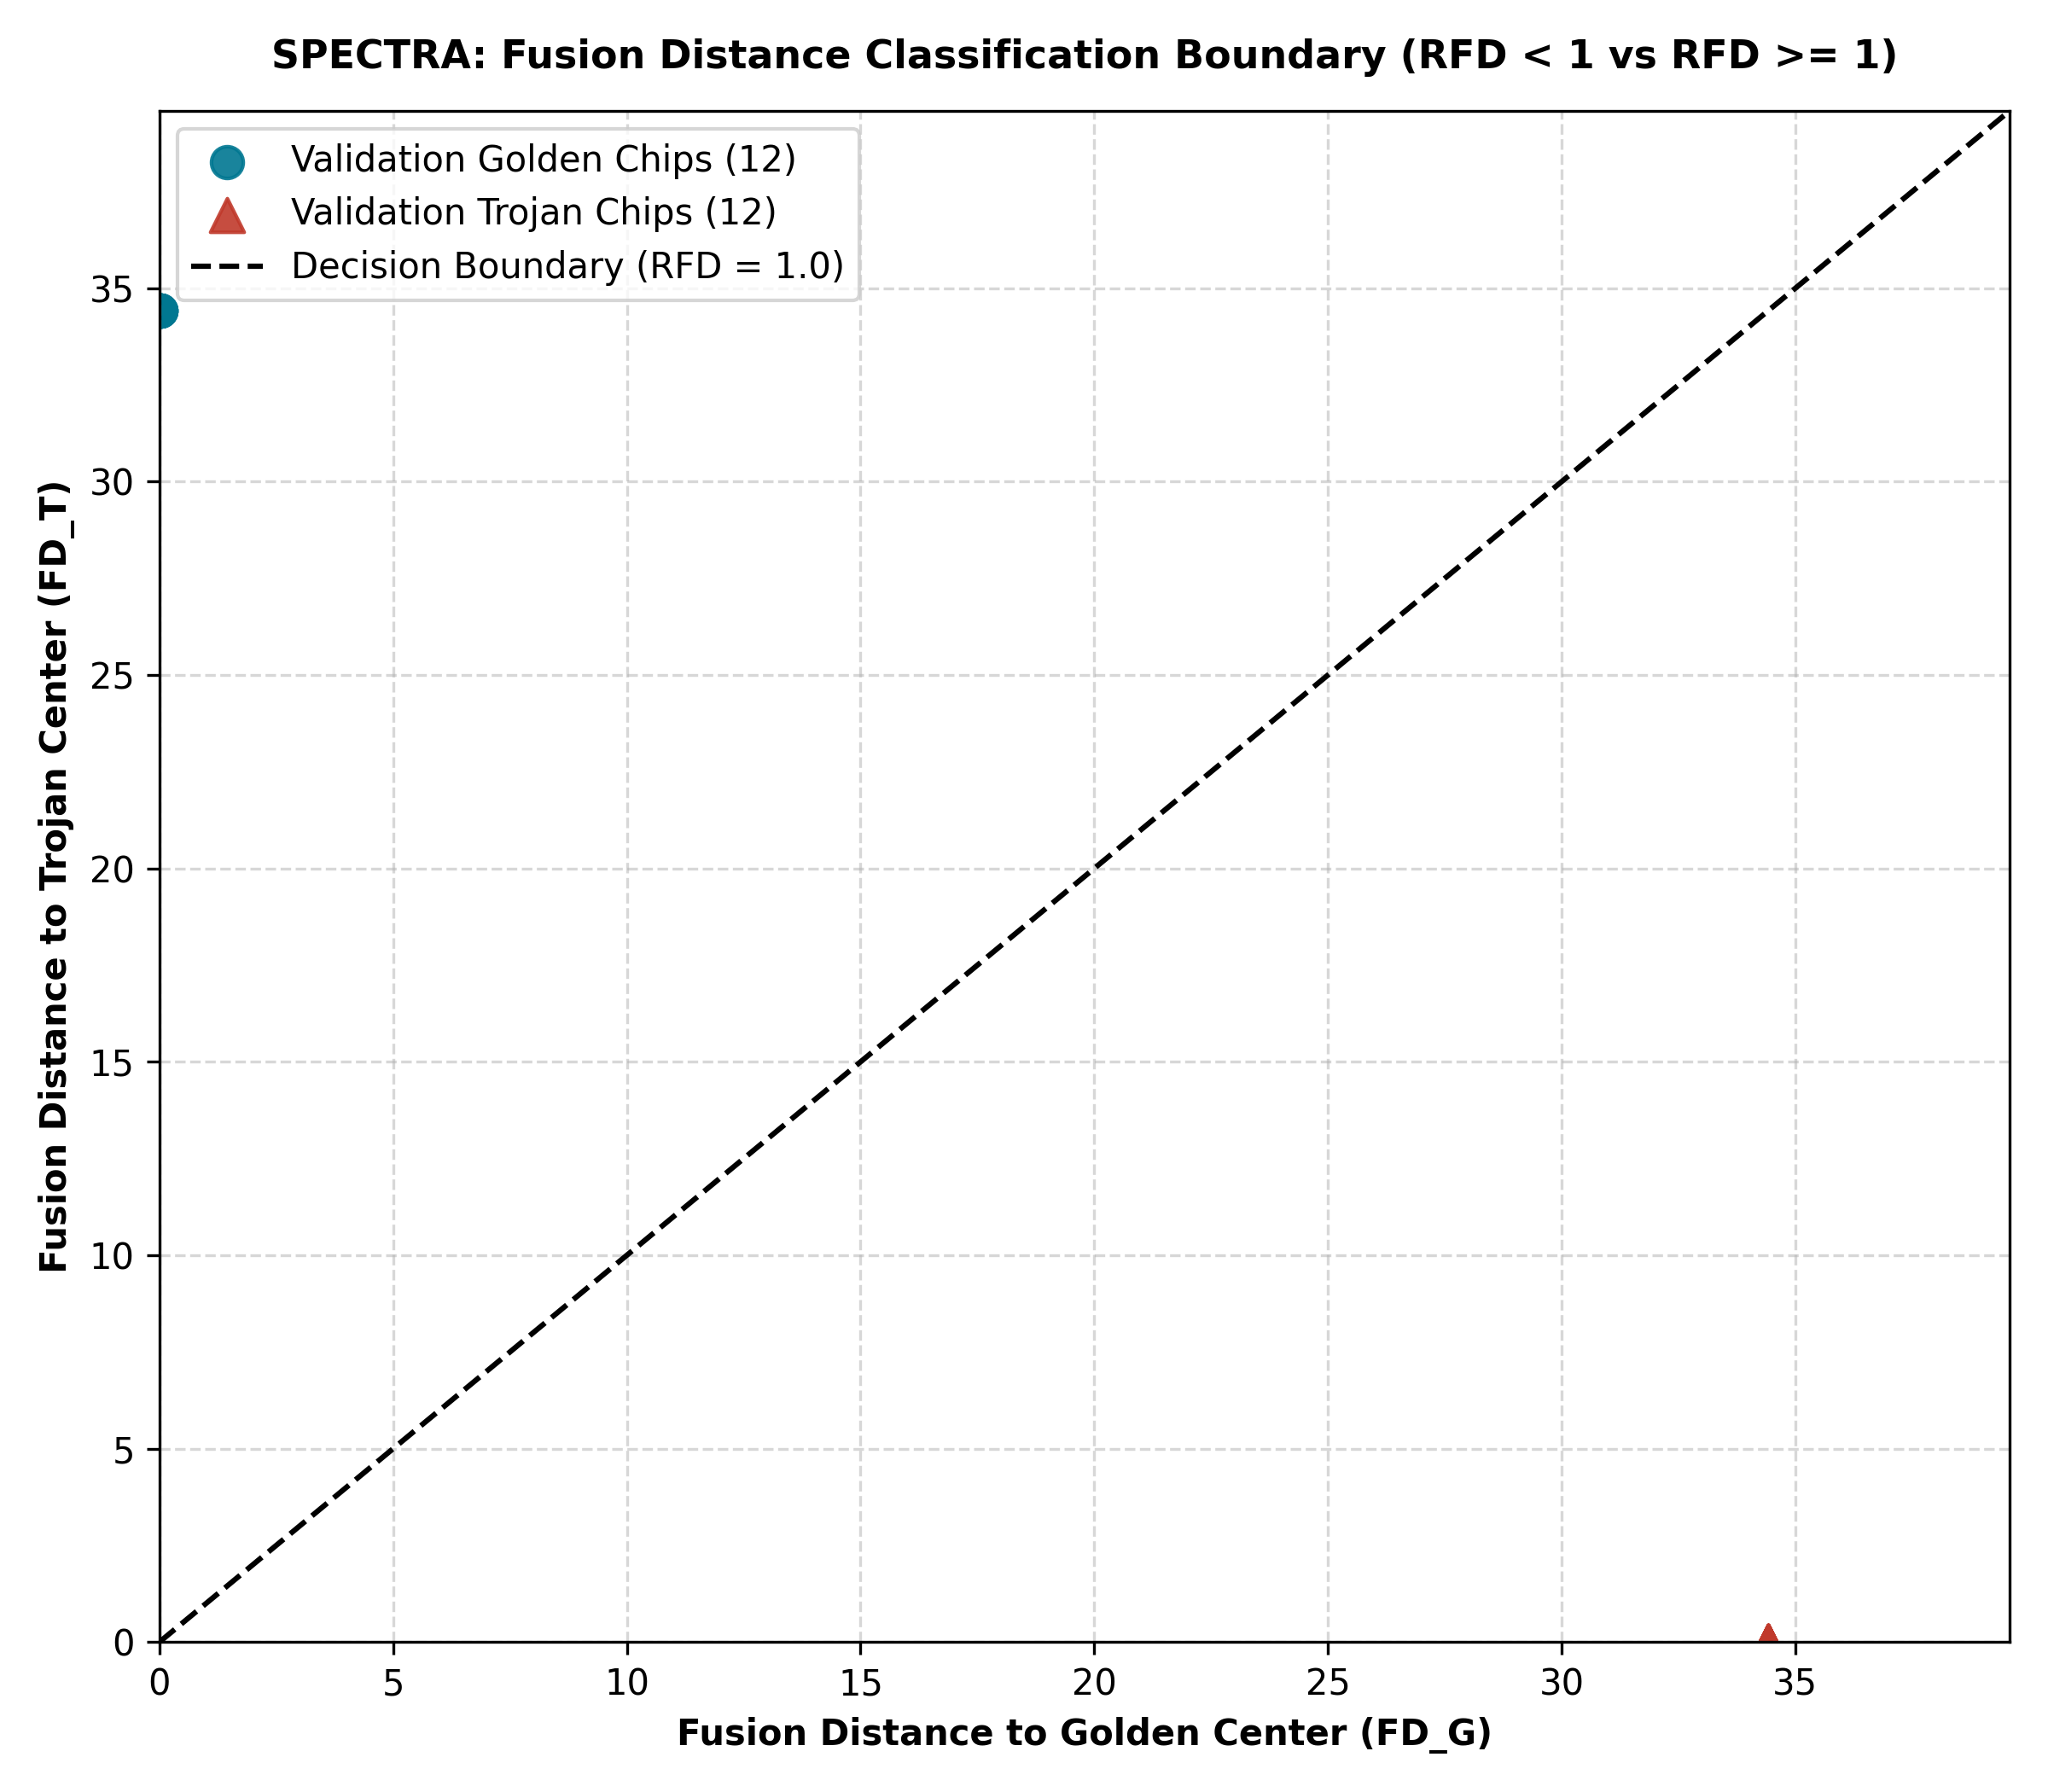
\includegraphics[width=\linewidth, height=2.20cm, keepaspectratio]{screenshots/fusion_distance_classification.png}
      \end{imagebox}
      \vspace{1.5pt}
      {\fontsize{7.5pt}{9.5pt}\selectfont\itshape\color{black!80}
      \textbf{Preliminary Data: Massive Separation Expansion:}\\
      With entropy weighting, Golden dies achieve $R_{FD} \approx 2.78 \times 10^{-4} \ll 1.0$ while Trojan dies achieve $R_{FD} \approx 3762.58 \gg 1.0$. The dynamic separation ratio expands to \textbf{$> 1.35 \times 10^7$} (over 6 orders of magnitude beyond the base paper)!\par}
    \end{column}
  \end{columns}
\end{frame}

% -----------------------------------------------------------------------------
% SLIDE 12: ROADMAP TOWARD EVALUATION 2 & PUBLICATION PLAN
% -----------------------------------------------------------------------------
\begin{frame}[t]
  \slideheader{ROADMAP TOWARD EVALUATION 2 \& PUBLICATION}
  \vspace*{-0.18cm}

  \begin{columns}[T, onlytextwidth]
    \begin{column}{0.485\textwidth}
      \begin{glassbox}[top=2pt, bottom=2pt, left=6pt, right=6pt, title={Completed vs.\ Planned Milestones}]{}
        \textbf{Phase 1: Base Paper Replication [DONE]:}
        \begin{itemize}\setlength{\itemsep}{1pt}
          \item[$\checkmark$] 100\% faithful Verilog RTL core and counter Trojan.
          \item[$\checkmark$] Python pipeline reproducing Eqs.\ 1--20 with 100\% accuracy.
          \item[$\checkmark$] Replicated Figs.\ 6--9 matching published paper 1:1.
        \end{itemize}
        \vspace{1.5pt}

        \textbf{Phase 2: Novelty Validation (Evaluation 2):}
        \begin{itemize}\setlength{\itemsep}{1pt}
          \item[$\square$] AWGN sweep ($30\text{ dB} \to 5\text{ dB}$) and clock drift ($\pm 3\%$) for AHBE.
          \item[$\square$] Multi-benchmark generalization (AES-T100, T400, T800).
          \item[$\square$] Hardware implementation on 28nm Artix-7 FPGA.
        \end{itemize}
      \end{glassbox}
    \end{column}

    \begin{column}{0.485\textwidth}
      \begin{glassbox}[top=2pt, bottom=2pt, left=6pt, right=6pt, title={Publication \& Defense Trajectory}]{}
        \textbf{Target Publication Venues:}
        \begin{itemize}\setlength{\itemsep}{1pt}
          \item \textit{IEEE Trans.\ Inf.\ Forensics \& Security} (TIFS).
          \item \textit{IEEE Internet of Things Journal} (JIOT).
          \item IEEE Int.\ Symp.\ on Hardware Oriented Security (HOST).
        \end{itemize}
        \vspace{1.5pt}

        \textbf{Key Manuscript Contributions:}
        \begin{itemize}\setlength{\itemsep}{1pt}
          \item Rigorous mathematical proof of single-bin fragility.
          \item Continuous AHBE band energy integration algorithm.
          \item Information-entropy adaptive distance fusion.
        \end{itemize}
      \end{glassbox}
    \end{column}
  \end{columns}
\end{frame}

% -----------------------------------------------------------------------------
% SLIDE 13: THANK YOU & QUESTIONS
% -----------------------------------------------------------------------------
\begin{frame}[t]
  \slideheader{THANK YOU \& QUESTIONS}
  \vspace*{-0.05cm}

  \begin{center}
    \begin{glasscard}[width=0.92\linewidth, arc=3.5mm, top=12pt, bottom=12pt, left=15pt, right=15pt]
      \centering
      \vspace{0.15cm}
      {\fontsize{18pt}{22pt}\selectfont\bfseries\color{textPrimary} Thank You!}\\[8pt]
      {\color{accentDark}\rule[3pt]{0.16\linewidth}{1.2pt}}\\[8pt]
      {\fontsize{10.5pt}{13.5pt}\selectfont\bfseries\color{accentDark} Hardware Security and Trust (23ECE341)}\\[6pt]
      {\fontsize{9.5pt}{11.5pt}\selectfont\color{textPrimary} Open for Questions, Evaluation Feedback \& Technical Discussion}\\[12pt]
      \begin{tikzpicture}
        \node[draw=accentDark!50, line width=0.8pt, rounded corners=3pt, fill=white, fill opacity=0.85, text opacity=1, inner xsep=16pt, inner ysep=6pt]{%
          {\fontsize{8.5pt}{11.0pt}\selectfont\color{textPrimary}
          \textbf{Project Team:}\hspace{0.5em} Chandan Sai Pavan Padala \quad$\bullet$\quad M Madhumitha \quad$\bullet$\quad M V Sri Harsha}%
        };
      \end{tikzpicture}\\[10pt]
      {\fontsize{8.0pt}{10.0pt}\selectfont\color{black!75} Under the Guidance of \textbf{\color{textPrimary}\guideName}}\\[3pt]
      {\fontsize{7.5pt}{9.5pt}\selectfont\color{black!60} Department of Electronics and Communication Engineering \quad$\bullet$\quad Amrita Vishwa Vidyapeetham}
      \vspace{0.15cm}
    \end{glasscard}
  \end{center}
\end{frame}

\end{document}
